%   Filename    : chapter_4.tex 

\chapter{Results and Discussions}
This chapter presents the results from the machine learning and deep learning analyses conducted on the preprocessed dataset. It includes an evaluation of various machine learning classifiers and the application of deep learning models for image-based classification. The primary focus is on identifying key predictors and assessing classification performance for sex identification in \textit{T. granosa}.

\section{Machine Learning Analysis}

This chapter outlines the results of preprocessing, training of machine learning models, and feature importance analysis, all conducted in Google Colab using Python. The dataset was preprocessed in Colab, and the training and evaluation of various classifiers were performed entirely within this environment.  This part of the paper includes five subsections: data exploration, statistical analysis, feature importance analysis, performance evaluation, and visualizations for machine learning.

\subsection{Data Exploration}

Exploratory data analysis was performed to characterize the dataset using data to understand underlying patterns and behaviors using descriptive statistics and correlation heatmap. A correlation heatmap was created to assess the relationship between the predictors and the target variable.

The heatmap (\textit{see Figure~\ref{fig:heatmap}}) revealed three features most correlated with the sex of \textit{T. granosa}: the width-height ratio (r = 0.18), the umbos distance-length ratio (r = 0.12), and the distance between the umbos (r = 0.12). Each of these features demonstrated a weak positive relationship with the target variable. 

\vspace{0.5cm}
\begin{figure}[!htbp]
	\centering
	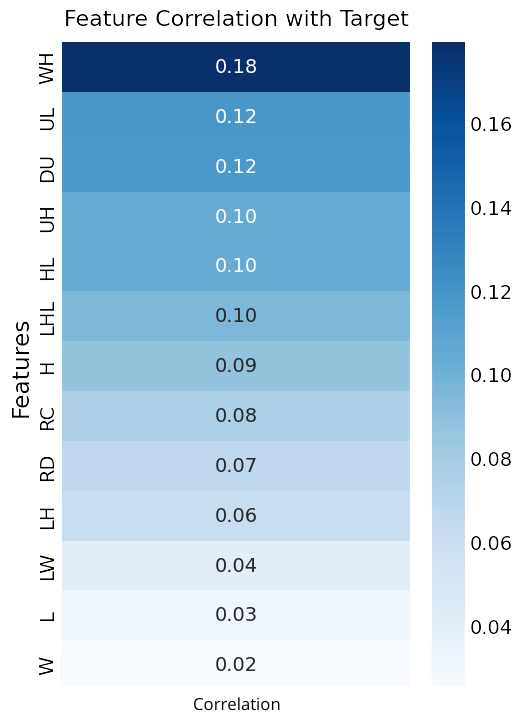
\includegraphics[width=0.4\textwidth]{figures/heatmap.png}
	\caption{Heatmap of morphometric correlations with \textit{T. granosa} sex.}
	\label{fig:heatmap}
\end{figure}

\newpage
\subsection{Statistical Analysis}

\textbf{\textit{Descriptive Statistics}}

Descriptive statistics summarize and describe the main characteristics of a dataset, offering a concise overview of its features. Table~\ref{tab:morphometric-comparison}  provides a comparison of the morphometric features of \textit{T. granosa} between male and female samples. Generally, male \textit{T. granosa} have slightly longer shells (mean = 51.69 mm) than females (mean = 50.24 mm). However, female \textit{T. granosa} exhibits marginally greater shell height and width. These observations suggest that male shells are more elongated, while female shells appear more rounded or inflated.

The rib count and rib density are nearly identical between the sexes, indicating that these features might not be significant indicators for distinguishing between males and females. However, noticeable differences are observed in hinge line length and the distance between umbos. Female \textit{T. granosa} exhibits longer hinge lines (mean = 31.97 mm) and a greater umbo distance (mean = 4.05 mm) than males, which could point to structural differences in shell formation related to sex.

In terms of the shape of \textit{T. granosa}, the calculated ratios offer additional insight. Males have slightly higher length-to-width and length-to-height ratios, reinforcing that their shells are more elongated. In contrast, females exhibit slightly higher umbo-related ratios, such as umbo distance-to-height and umbo distance-to-length, suggesting a more prominent umbo or hinge area.

Looking at the standard deviations, male specimens demonstrate greater variability in certain features—particularly in shell length, where the standard deviation is notably higher (31.75) than that of females (7.49). This suggests that male \textit{T. granosa} exhibits a wider range of sizes. While the differences are subtle, features like shell length, hinge line length, and specific shape ratios may be useful inputs for developing a machine learning model for sex classification.

\vspace{0.5cm}
\begin{table}[H]
	\centering
	\small
	\begin{tabular}{lcccc}
		\hline
		\textbf{Feature} & \textbf{Male Mean} & \textbf{Female Mean} & \textbf{Male SD} & \textbf{Female SD} \\ \hline
		Length & 51.69 & 50.24 & 31.75 & 7.49 \\
		Width & 37.69 & 37.95 & 5.13 & 5.66 \\
		Height & 33.85 & 34.74 & 4.98 & 5.18 \\
		Rib Count & 19.87 & 19.74 & 0.85 & 0.84 \\
		Hinge Line Length & 30.81 & 31.97 & 5.96 & 6.27 \\
		Umbos Distance & 3.50 & 4.05 & 1.50 & 3.08 \\
		LW Ratio & 1.39 & 1.33 & 1.06 & 0.08 \\
		LH Ratio & 1.54 & 1.45 & 0.98 & 0.08 \\
		WH Ratio & 1.11 & 1.09 & 0.07 & 0.06 \\
		UL Ratio & 0.07 & 0.08 & 0.02 & 0.06 \\
		HL Ratio & 0.62 & 0.63 & 0.07 & 0.06 \\
		UH Ratio & 0.10 & 0.12 & 0.04 & 0.09 \\
		Rib Density & 0.40 & 0.40 & 0.06 & 0.06 \\ \hline
	\end{tabular}
	\caption{Comparison of morphometric features between male and female \textit{T. granosa}, showing mean and standard deviation (SD) values.}
	\label{tab:morphometric-comparison}
\end{table}

\textbf{\textit{Mann-Whitney U Test}}

As part of the exploratory data analysis, statistical testing confirmed that the dataset did not follow a normal distribution (\textit{see Table~\ref{tab:mann-whitney}}). Consequently, the Mann-Whitney U test was applied with a significance level of $\alpha = 0.05$ to compare male and female samples. Out of thirteen features, five showed statistically significant differences. These included: width-height ratio ($p = 0.003$), length-width ratio ($p = 0.011$), umbos distance-length ratio ($p = 0.019$), distance between umbos ($p = 0.025$), and umbos distance-height ratio ($p = 0.036$). 

It is important to note that statistical significance does not imply predictive importance. Therefore, further analysis, such as feature importance evaluation, was performed to identify the most informative predictors for classification.

\vspace{0.5cm}
\begin{table}[H]
	\centering
	\small % or \footnotesize or \scriptsize
	\begin{tabular}{lc}
		\hline
		\textbf{Variable} & \textbf{p-value} \\ \hline
		WH\_ratio & 0.003 \\
		LW\_ratio & 0.011 \\
		UL\_ratio & 0.019 \\
		Distance Umbos & 0.025 \\
		UH\_ratio & 0.036 \\
		HL\_ratio & 0.079 \\
		Length (Hinge Line) & 0.120 \\
		Height & 0.124 \\
		Rib Density & 0.181 \\
		Rib count & 0.251 \\
		Length & 0.334 \\
		LH\_ratio & 0.490 \\
		Width & 0.753 \\ \hline
		
	\end{tabular}
	
	\caption{Mann-Whitney U test results for sex-based feature comparison.}
	\label{tab:mann-whitney}
\end{table}

%\newpage
\subsection{Feature Importance Analysis}

Feature importance was assessed using the Kruskal-Wallis test, a non-parametric method that is suitable for evaluating differences in distributions across groups when the data does not follow a normal distribution. This approach was chosen because of the non-normality of the dataset and its robustness in handling continuous and ordinal data without assuming homogeneity of variances. \cite{ribeiro2024}

Kruskal-Wallis test analysis showed that the width-to-height ratio (WH ratio) had the highest importance score, indicating it is the most statistically significant feature for distinguishing the sex of \textit{T. granosa}. Other notable features included the length-to-width ratio (LW ratio), umbos distance-to-length ratio (UL ratio), distance between the umbos, and umbos distance-to-height ratio (UH ratio), all of which contributed significantly to the classification task (\textit{refer to Figure~\ref{fig:kw}}).

\begin{figure}[!htbp]
	\centering
	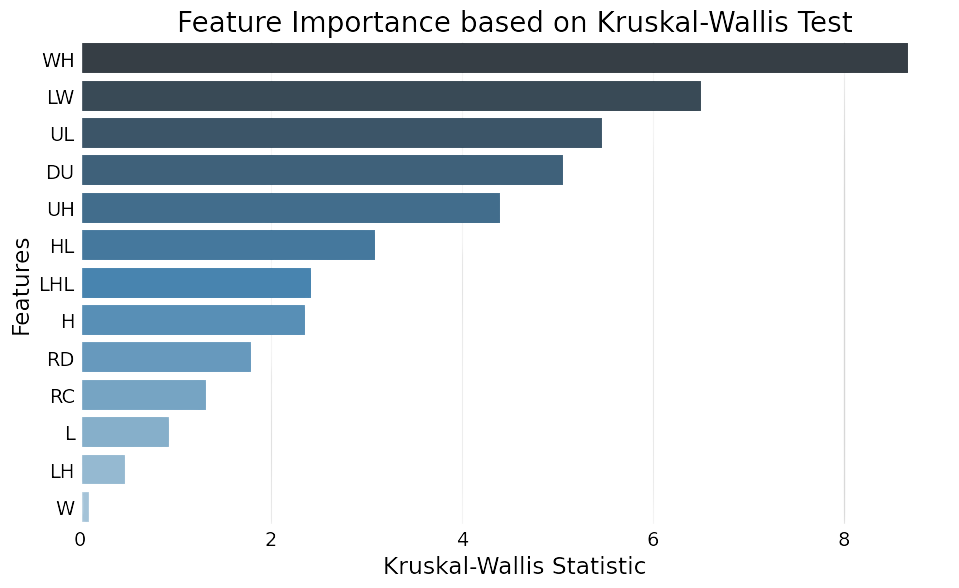
\includegraphics[width=0.8\textwidth]{figures/kw.png}
	\caption{Feature importance scores using the Kruskal-Wallis test.}
	\label{fig:kw}
\end{figure}

\subsection{Performance Evaluation}
\label{tab:performance-eval}

Table~\ref{tab:performance-13-features} shows the performance metrics of different machine learning models trained using all 13 features from the dataset. Among the models, Gradient Boosting achieved the highest accuracy of 61.03\%, along with strong precision, recall, and F1 Score values. AdaBoost also performed competitively, with an accuracy of 60.63\%. These results highlight the effectiveness of ensemble methods such as Gradient Boosting and AdaBoost when utilizing the full feature set, likely because of their capability to combine multiple weak learners into a more robust predictive model \cite{hussain2024}.  

\begin{table}[H]
	\centering
	\resizebox{\textwidth}{!}{
		\begin{tabular}{lcccccc}
			\hline
			\textbf{Model} & \textbf{Accuracy (\%)} & \textbf{Precision (\%)} & \textbf{Recall (\%)} & \textbf{F1 Score (\%)} \\ \hline
			Support Vector Machine   & 58.62 & 58.62 & 58.62 & 58.44 \\
			Logistic Regression      & 57.83 & 57.83 & 57.83 & 57.61 \\
			K-Nearest Neighbors      & 51.18 & 51.31 & 51.18 & 50.77 \\
			Extra Trees              & 59.07 & 59.54 & 59.07 & 58.45 \\
			Random Forest            & 59.85 & 59.99 & 59.85 & 59.80 \\
			\cellcolor{celadon}Gradient Boosting        & \cellcolor{celadon}61.03 & \cellcolor{celadon}61.32 & \cellcolor{celadon}61.03 & \cellcolor{celadon}60.81 \\
			AdaBoost & 60.63 & 60.98 & 60.63 & 60.39 \\
			\hline
		\end{tabular}
	}
	\caption{Performance metrics for models with all 13 features.}
	\label{tab:performance-13-features}
\end{table}

Table~\ref{tab:performance-5-features} presents the performance of the same models using only the top five features identified through Kruskal-Wallis feature importance analysis. The selected features are the distance between the umbos, length-to-width ratio, width-to-height ratio, umbos distance-to-height ratio, and umbos distance-to-length ratio.

Interestingly, the overall performance of the models improved when using only the top 5 features compared to using all 13. KNN achieved the best results with an accuracy of 64.16\%, precision of 64.97\%, recall of 64.16\%, and an F1 Score of 63.75\%. Gradient Boosting followed closely behind. These findings suggest that reducing the feature set to the most relevant variables helped simplify the models, improved generalization, and enhanced predictive performance—particularly for KNN, which showed a notable improvement over its earlier results with the full feature set.

\vspace{0.5 cm}
\begin{table}[H]
	\centering
	\resizebox{\textwidth}{!}{
		\begin{tabular}{lcccccc}
			\hline
			\textbf{Model} & \textbf{Accuracy (\%)} & \textbf{Precision (\%)} & \textbf{Recall (\%)} & \textbf{F1 Score (\%)} \\ \hline
			Support Vector Machine   & 63.77 & 64.47 & 63.77 & 63.42 \\
			Logistic Regression      & 63.75 & 63.87 & 63.75 & 63.70 \\
			\cellcolor{celadon}K-Nearest Neighbors      & \cellcolor{celadon}64.16 & \cellcolor{celadon}64.97 & \cellcolor{celadon}64.16 & \cellcolor{celadon}63.75 \\
			Extra Trees              & 61.04 & 61.68 & 61.04 & 60.67 \\
			Random Forest            & 61.01 & 61.12 & 61.01 & 60.91 \\
			Gradient Boosting        & 64.15 & 64.24 & 64.15 & 64.01 \\
			AdaBoost                 & 61.02 & 61.26 & 61.02 & 60.82 \\
			\hline
		\end{tabular}
	}
	\caption{Performance metrics for models with 5 features.}
	\label{tab:performance-5-features}
\end{table}

\subsection{Visualizations for Machine Learning}

Figure~\ref{fig:cm_ml} is a confusion matrix that summarizes the performance of the KNN model in classifying \Tgranosa based on their sex, where 0 represents female samples and 1 represents male samples. From the matrix, it can be observed that out of all the actual female samples (true label 0), 91 were correctly predicted as female (true positive for class 0), while 36 were incorrectly classified as male (false negative for class 0). On the other hand, out of all the actual male samples (true label 1), 72 were correctly predicted as male (true positive for class 1), while 55 were incorrectly classified as female (false negative for class 1).

These classification results can be partially accounted for by the descriptive morphometric feature statistics. From Table~\ref{tab:morphometric-comparison}, female samples of \textit{T. granosa} have more uniform and lower variance measurements than males, particularly in such features as shell length (SD = 7.49 for females vs. 31.75 for males). This reduced variability indicates that female samples constitute a closer group in feature space, thus are simpler for KNN to correctly classify. By comparison, the greater variation of male samples will most likely render them more spread out and vulnerable to overlap with female data. In addition, certain shape features (e.g., height, width, rib density) exhibit little variation between sexes and may thus make it more difficult for the model to differentiate between long male shells and curved female shells when the male values are closer to female means. These are some of the possible reasons why the model records a greater true positive value for females and false negatives for males.

\begin{figure}[!htbp]
	\centering
	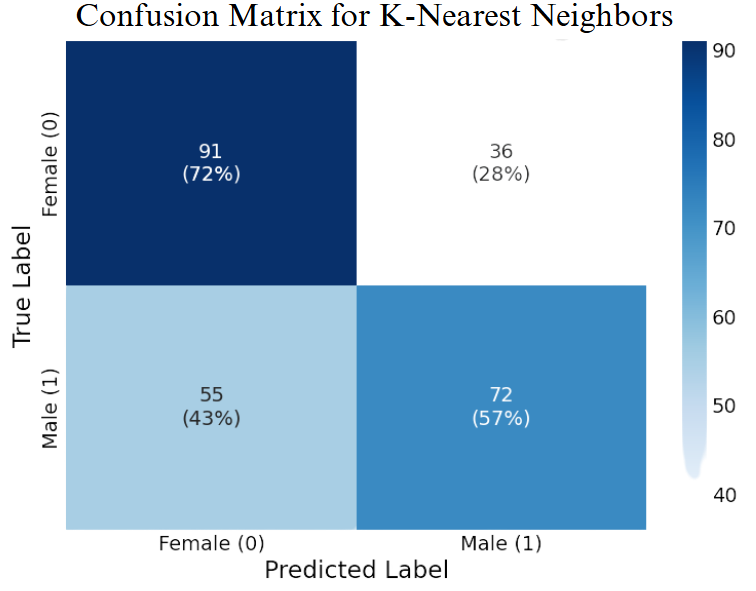
\includegraphics[width=0.8\textwidth]{figures/confusion_matrix_ml.png}
	\caption{KNN confusion matrix for \textit{T. granosa} sex classification.}
	\label{fig:cm_ml}
\end{figure}

\newpage
Figure~\ref{fig:roc_ml} displays the average receiver operating characteristic (ROC) curve, showing KNN’s ability to distinguish between positive and negative cases. The ROC curve helps assess the trade-off between sensitivity (true positive rate) and specificity (1 - false positive rate). The area under the curve (AUC) value, which ranges from 0.5 (random chance) to 1 (perfect discrimination), is used to evaluate the model’s overall performance. In this case, KNN achieved an average AUC of 0.7004, indicating that it performs better than random guessing and has reasonable predictive ability.

\begin{figure}[!htbp]
	\centering
	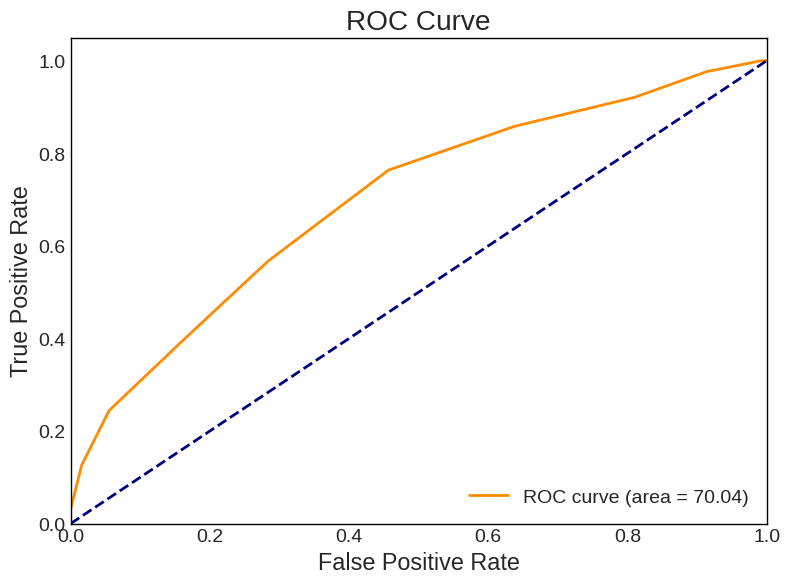
\includegraphics[width=0.8\textwidth]{figures/roc_ml.png}
	\caption{ROC curve with AUC score for KNN.}
	\label{fig:roc_ml}
\end{figure}

\newpage
\section{Deep Learning Analysis}
This section presents the performance of the convolutional neural network (CNN) model in classifying the sex of \Tgranosa based on shell morphology. The analysis evaluates the model's ability to distinguish between male and female shell images using various evaluation metrics. This part of the paper includes six subsections: baseline model, comparison of individual and combined angles, training result and hyperparameter tuning, proposed model, learning rates and training behavior per fold, and visualizations for deep learning.

The machine learning analysis (\textit{see Figure~\ref{tab:performance-5-features}}) revealed that five of the original features produced significant results. The k-nearest neighbors (KNN) model achieved an accuracy of 64.16\%, precision of 64.97\%, recall of 64.16\%, and an F1 Score of 63.75\%. This section compares the model's performance across different angles based on the results of the machine learning and feature importance analysis.

\subsection{Baseline Model}
This section presents the baseline model with a batch size of 16 and 20 epochs, which will serve as the starting point for comparison and provide a guideline for hyperparameter tuning. The focus will be on one of the angles, specifically the Left Lateral view, since the feature importance analysis using the Kruskal-Wallis Test indicated that the width-to-height ratio had the highest importance score, which is most visible from the Left Lateral view.

The unbalanced dataset, which consisted of 144 male samples and 127 female samples, achieved an accuracy of 65.27\%, precision of 71.82\%, recall of 58.99\%, an F1 Score of 63.99\%, an AUC score of 73.08\%, and a loss of 0.6122. However, to address the class imbalance and enhance model performance, random undersampling was performed. This approach resulted in improved performance metrics for the balanced dataset, with an accuracy of 67.34\%, precision of 69.43\%, a recall of 64.06\%, an F1 Score of 65.60\%, an AUC score of 74.31\%, and a lower loss of 0.5981.

%\vspace{-10pt}
\begin{table}[H]
	\centering
	\resizebox{\textwidth}{!}{
		\begin{tabular}{lcccccc}
			\hline
			\textbf{Dataset} & \textbf{Accuracy (\%)} & \textbf{Precision (\%)} & \textbf{Recall (\%)} & \textbf{F1 Score (\%)}  & \textbf{AUC score (\%)}  & \textbf{Loss} \\ \hline
			Imbalanced   & 65.27 & 71.82 & 58.99 & 63.99 & 73.08 & 0.6122 \\
			\rowcolor{celadon}Balanced     & 67.34 & 69.43 & 64.06 & 65.60 & 74.31 & 0.5981 \\
			\hline
		\end{tabular}
	}
	\caption{Performance metrics for balanced vs imbalanced datasets (Batch Size: 16, Epochs: 20).}
	\label{tab:unbalanced-balanced}
\end{table}

\subsection{Comparison of Individual and Combined Angles}

Using the same batch size and number of epochs, performance was compared across all individual angles and the combination of the two highest-performing angles based on accuracy, using a balanced dataset. For the combined analysis, samples from the two selected angles were placed side by side, and a new dataset folder was created for male and female samples. 

Table~\ref{tab:individual-combined} presents the performance metrics for each individual angle and the combination of the two highest-performing angles in terms of accuracy. The Left Lateral view achieved the highest accuracy (67.34\%) and precision (69.43\%), while the Dorsal view obtained the highest recall (77.88\%) and F1 Score (69.96\%). Meanwhile, the Ventral view recorded the highest AUC score (74.87\%), indicating its strong ability to distinguish between classes.
Combining the Ventral and Left Lateral views resulted in an overall accuracy of 62.60\%, suggesting that while combined images may provide complementary information, individual angle views still outperformed the combined views under the current experimental setup.

%\vspace{-15pt}
\begin{table}[H]
	\centering
	\resizebox{\textwidth}{!}{
		\begin{tabular}{lcccccc}
			\hline
			\textbf{Angle} & \textbf{Accuracy (\%)} & \textbf{Precision (\%)} & \textbf{Recall (\%)} & \textbf{F1 Score (\%)} & \textbf{AUC score (\%)} & \textbf{Loss} \\ \hline
			Dorsal 	 				& 66.54 & 63.76 & \cellcolor{celadon}77.88 & \cellcolor{celadon}69.96 & 73.09 & 0.6152 \\
			Ventral  				& 67.30 & 69.33 & 66.18 & 66.53 & \cellcolor{celadon}74.87 & 0.6159 \\
			Anterior  				& 51.57 & 31.11 & 6.31  & 10.02 & 65.87 & 0.6825 \\
			Posterior  				& 61.43 & 63.48 & 51.17 & 54.25 & 70.12 & 0.6257 \\
			Left Lateral  			& \cellcolor{celadon}67.34 & \cellcolor{celadon}69.43 & 64.06 & 65.60 & 74.31 & 0.5981 \\
			Right Lateral  			& 65.37 & 67.18 & 59.82 & 62.99 & 71.02 & 0.6115 \\
			Ventral + Left Lateral  & 62.60 & 67.02 & 57.85 & 58.57 & 70.37 & 0.6433 \\
			\hline
		\end{tabular}
	}
	\caption{Performance metrics for individual and combined angles (Batch Size: 16, Epochs: 20).}
	\label{tab:individual-combined}
\end{table}

\subsection{Training Result and Hyperparameter Tuning}
The Left Lateral angle view was selected for further optimization. Several experiments were conducted by tuning hyperparameters such as batch size, number of epochs, and activation functions. Each adjustment was compared against the baseline model to enhance performance and develop a robust CNN for sex classification of \textit{T. granosa}.

The Left Lateral angle was chosen because it achieved the highest accuracy and precision among all individual views, and because the Kruskal-Wallis feature importance analysis indicated that the width-to-height ratio, a feature most visible from the lateral perspective, was the most significant morphological trait for classification. Therefore, focusing on this view was expected to maximize the model's learning capacity and improve classification performance.

\noindent\textbf{A. Batch Size and Number of Epochs}

Table~\ref{tab:batchsize-epoch} shows the results indicating that a batch size of 32 with 50 epochs achieved the best overall performance, with an accuracy of 71.68\%, a precision of 72.52\%, a recall of 69.29\%, an F1 Score of 69.12\%, and AUC score of 77.34\%.

In contrast, increasing the batch size to 64 resulted in lower recall and F1 Scores, suggesting that smaller batch Sizes (16 or 32) are more effective for this dataset. A moderate batch size of 32 allowed the model to generalize better and maintain stable learning, while too large batch sizes may have led to underfitting.

\begin{table}[H]
	\centering
	\resizebox{\textwidth}{!}{
		\begin{tabular}{llccccccc}
			\hline
			\textbf{Epoch} & \textbf{Batch Size} & \textbf{Accuracy (\%)} & \textbf{Precision (\%)} & \textbf{Recall (\%)} & \textbf{F1 Score (\%)} & \textbf{AUC Score (\%)} & \textbf{Loss} \\
			\hline
			\multirow{3}{*}{20} 
			& 16 & 67.34 & 69.43 & 64.06 & 65.60 & 74.31 & 0.5981 \\
			& 32 & 68.13 & 72.25 & 58.95 & 62.34 & 74.76 & 0.6041 \\
			& 64 & 56.71 & 65.96 & 36.83 & 41.46 & 71.28 & 0.6692 \\
			\hline
			\multirow{3}{*}{30} 
			& 16 & 67.73 & 70.17 & 64.06 & 65.72 & 75.76 & 0.5900 \\
			& 32 & 71.28 & 73.17 & 66.89 & 68.27 & 76.76 & 0.5832 \\
			& 64 & 57.95 & 61.94 & 48.12 & 52.66 & 71.22 & 0.6241 \\
			\hline
			\multirow{3}{*}{50} 
			& 16 & 67.73 & 70.17 & 64.06 & 65.72 & 75.76 & 0.5900 \\
			& \cellcolor{celadon}32 & \cellcolor{celadon}71.68 & \cellcolor{celadon}72.52 & \cellcolor{celadon}69.29 & \cellcolor{celadon}69.12 & \cellcolor{celadon}77.34 & \cellcolor{celadon}0.5824 \\
			& 64 & 61.10 & 62.68 & 56.12 & 56.83 & 73.46 & 0.6086 \\
			\hline
		\end{tabular}
	}
	\caption{Effect of batch size and epoch values on CNN model performance.}
	\label{tab:batchsize-epoch}
\end{table}


\noindent\textbf{B. Activation Functions}

Table~\ref{tab:activation-function} shows the performance of different activation functions applied to the CNN model trained with a batch size of 32 and 50 epochs. Based on the results, the ReLU activation function achieved the best overall performance, with an accuracy of 71.68\%, precision of 72.52\%, recall of 69.29\%, F1 Score of 69.12\%, and AUC score of 77.34\%, along with the lowest loss at 0.5824. This suggests that ReLU remains an effective activation function for the classification of \textit{T. granosa}, outperforming both ELU and PReLU in this setup.

\vspace{0.2 cm}
\begin{table}[H]
	\centering
	\resizebox{\textwidth}{!}{
		\begin{tabular}{lcccccc}
			\hline
			\textbf{Activation Functions} & \textbf{Accuracy (\%)} & \textbf{Precision (\%)} & \textbf{Recall (\%)} & \textbf{F1 Score (\%)}  & \textbf{AUC score (\%)}  & \textbf{Loss} \\ \hline
			\rowcolor{celadon}ReLU  & 71.68 & 72.52 & 69.29 & 69.12  & 77.34 & 0.5824 \\
			ELU   					& 53.14 & 32.91 & 53.08 & 39.95  & 58.23 & 0.6796 \\
			PreLU   				& 62.64 & 66.59 & 50.43 & 56.96  & 72.33 & 0.6162 \\
			\hline
		\end{tabular}
	}
	\caption{Performance metrics for different activation functions (Batch Size: 32, Epochs: 50).}
	\label{tab:activation-function}
\end{table}

\subsection{Proposed Model}
This section presents the performance evaluation of the proposed convolutional neural network (CNN) model, trained with a batch size of 32, 50 epochs, and using the ReLU activation function. The model’s effectiveness was assessed through 5-fold cross-validation to ensure robustness and generalizability across different data partitions. 

The proposed model consistently achieved high performance in Folds 1, 3, and 5, with accuracy above 76\%, and strong recall and AUC scores, demonstrating its potential for reliable sex identification of \textit{T. granosa}. The mean standard deviation for the performance metrics is 71.68 $\pm$7.32 for accuracy,  71.68 $\pm$ 7.32 for precision, 72.52 $\pm$ 0.02 for recall, 72.52 $\pm$ 0.02 for F1 score, and 69.29 $\pm$ 0.22 for AUC score. The standard deviation indicates the spread and variability in the performance. All metrics show a good indication of spread and consistency across folds. However, some with higher standard deviation values are recall, and F1 indicates some inconsistencies in predicting positive classes across the folds. 

The slight variation in performance across folds may be attributed to differences in data distribution, emphasizing the importance of further data augmentation and balancing for future work.

\vspace{0.5 cm}
\begin{table}[H]
	\centering
	\resizebox{\textwidth}{!}{
		\begin{tabular}{lcccccc}
			\hline
			\textbf{Fold no.} & \textbf{Accuracy (\%)} & \textbf{Precision (\%)} & \textbf{Recall (\%)} & \textbf{F1 Score (\%)}  & \textbf{AUC score (\%)}  & \textbf{Loss} \\ \hline
			Fold 1  & 76.47 & 70.59 & 92.31 & 80.00  & 73.08 & 0.5975 \\
			Fold 2  & 62.75 & 70.59 & 46.15 & 55.81  & 71.85 & 0.6202 \\
			Fold 3  & 78.43 & 75.00 & 84.00 & 79.25  & 84.92 & 0.5392 \\
			Fold 4  & 62.75 & 71.43 & 40.00 & 51.28  & 71.08 & 0.6331 \\
			Fold 5  & 78.00 & 75.00 & 84.00 & 79.25  & 85.76 & 0.5219 \\
			\textbf{Mean $\pm$ SD} & 71.68 $\pm$ 7.32 & 72.52 $\pm$ 2.05 & 69.29 $\pm$ 21.71 & 69.12 $\pm$ 12.80 & 77.34 $\pm$ 6.57 & 0.5824 $\pm$ 0.04 \\
			\hline
		\end{tabular}
	}
	\caption{Per-fold performance metrics (Batch Size: 32, Epochs: 50, Activation Function: ReLU) and corresponding mean and standard deviation.}
	\label{tab:per-fold}
\end{table}



\vspace{0.75cm}
\begin{minipage}{\linewidth}
	\subsection{Learning Rates and Training Behavior per Fold}
\end{minipage}

This section presents the learning rate adjustments, early stopping events, and best epoch selections for each fold during the 5-fold cross-validation of the proposed model. During training, the ReduceLROnPlateau callback was employed to monitor the validation loss and automatically reduce the learning rate when performance plateaued. Additionally, EarlyStopping was utilized to halt training once no further improvement was observed after a set patience, and the model weights were restored from the end of the best-performing epoch to ensure optimal performance.

The following table summarizes the epochs where learning rate reductions occurred, the adjusted learning rates, the epochs at which early stopping took place, and the best epochs from which model weights were restored for each fold.

\vspace{0.5 cm}
\begin{table}[H]
	\centering
	\resizebox{\textwidth}{!}{
		\begin{tabular}{lcccc}
			\hline
			\textbf{Fold no.} & \begin{tabular}[c]{@{}c@{}}\textbf{Epoch}\\\textbf{(LR Reduced)}\end{tabular} & \begin{tabular}[c]{@{}c@{}}\textbf{Learning Rate}\\\textbf{After Reduction}\end{tabular} & \begin{tabular}[c]{@{}c@{}}\textbf{Early}\\\textbf{Stopping Epoch}\end{tabular} & \begin{tabular}[c]{@{}c@{}}\textbf{Best Epoch}\\\textbf{(Restored)}\end{tabular} \\ \hline
			Fold 1 & \begin{tabular}[c]{@{}c@{}}20\\23\end{tabular} & \begin{tabular}[c]{@{}c@{}}0.0005000\\0.0002500\end{tabular} & 25 & 17 \\ \hline
			Fold 2 & \begin{tabular}[c]{@{}c@{}}9\\14\\17\end{tabular} & \begin{tabular}[c]{@{}c@{}}0.0005000\\0.0002500\\0.0001250\end{tabular} & 19 & 11 \\ \hline
			Fold 3 & \begin{tabular}[c]{@{}c@{}}15\\18\end{tabular} & \begin{tabular}[c]{@{}c@{}}0.0005000\\0.0002500\end{tabular} & 20 & 12 \\ \hline
			Fold 4 & \begin{tabular}[c]{@{}c@{}}12\\15\\27\\30\end{tabular} & \begin{tabular}[c]{@{}c@{}}0.0005000\\0.0002500\\0.0001250\\0.0000625\end{tabular} & 32 & 24 \\ \hline
			Fold 5 & \begin{tabular}[c]{@{}c@{}}20\\23\end{tabular} & \begin{tabular}[c]{@{}c@{}}0.0005000\\0.0002500\end{tabular} & 25 & 17 \\ \hline
		\end{tabular}
	}
	\caption{Learning rate reductions, early stopping, and best epochs per fold during 5-fold cross-validation.}
	\label{tab:learning-folds}
\end{table}


\subsection{Visualizations for Deep Learning}

Figure~\ref{fig:tvapf} shows the performance of the model in the training and validation in terms of accuracy across five folds. The graph across folds displays a consistent upward trend for the training accuracy. However, there is an observable change in the performance, particularly in Folds 1 and 2, where it shows a slight downward trend in the validation accuracy.

\begin{figure}[!htbp]
	\centering
	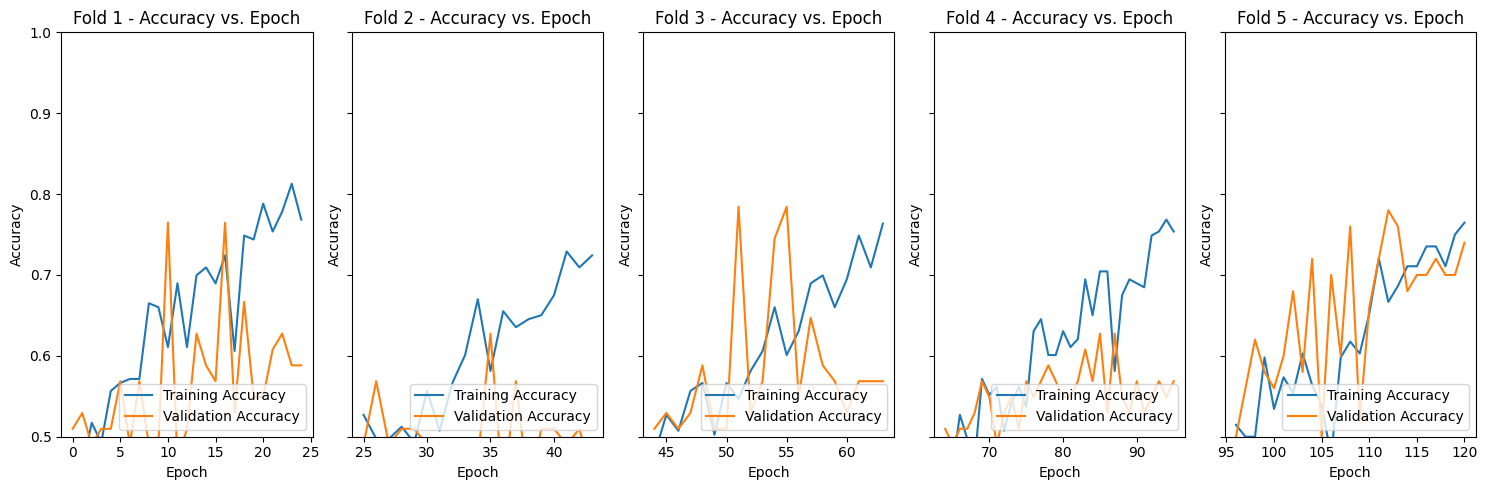
\includegraphics[width=0.8\textwidth]{figures/acc_epoch.png}
	\caption{Training and validation accuracy per fold.}
	\label{fig:tvapf}
\end{figure}

\newpage
Figure~\ref{fig:atvaaf} shows the average performance of the model in terms of training and validation accuracy across five folds. An upward trend is observable in the training and validation accuracy, indicating that the model gradually improves over the epochs. While fluctuations or dips can be seen in the validation accuracy, the model recovers in later epochs. The training accuracy remains consistently higher than the validation accuracy, which is expected behavior, as it learns from the training data. Generally, the model demonstrates a gradual improvement in learning, as reflected in the average upward trend aggregated across five folds.

\begin{figure}[!htbp]
	\centering
	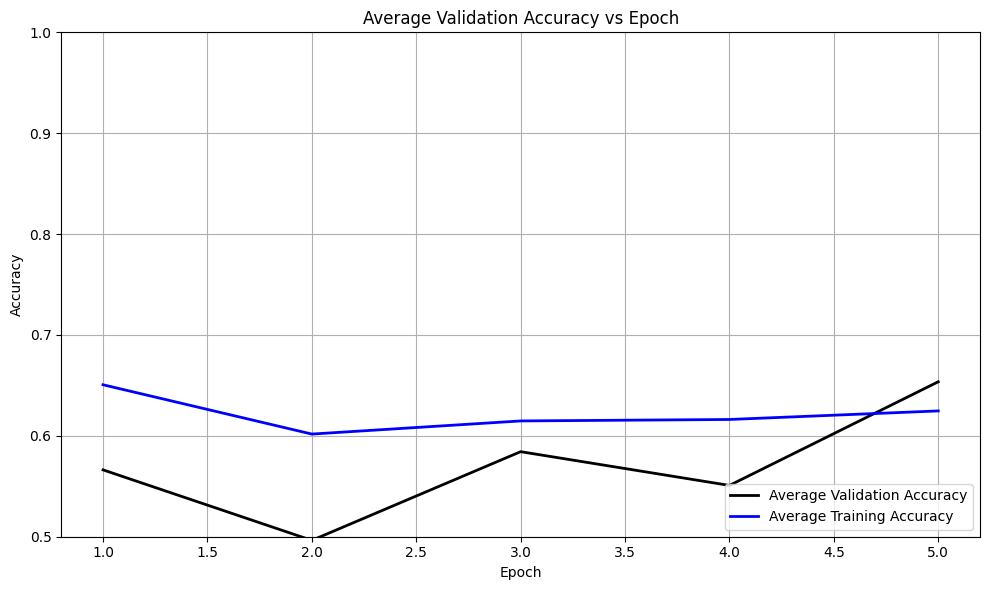
\includegraphics[width=0.8\textwidth]{figures/avg_acc.png}
	\caption{Average training and validation accuracy across folds.}
	\label{fig:atvaaf}
\end{figure}

Figure~\ref{fig:tvlpf} shows the performance of the model in the training and validation in terms of the training and validation loss across five folds. The graph across folds displays a consistent downward trend for the training loss. On the other hand, there is an observable change in the performance, especially in Folds 1,2,3, and 4, where it shows an upward trend in the validation loss. This is an implication for the learning performance of the model, as it may not be learning effectively. 

\begin{figure}[!htbp]
	\centering
	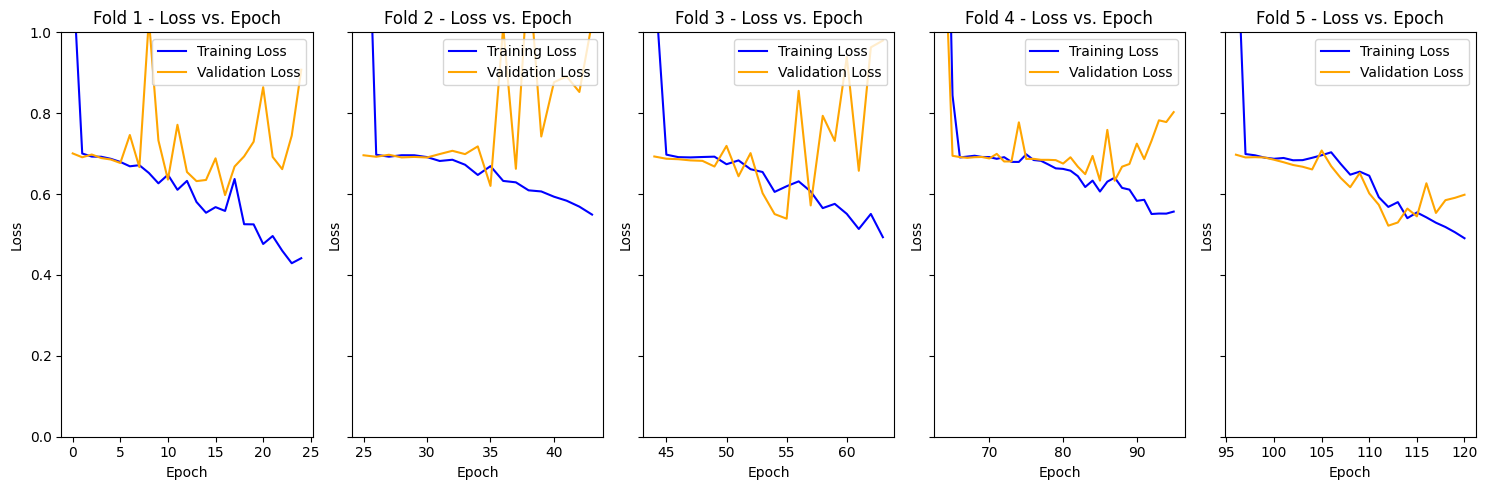
\includegraphics[width=0.8\textwidth]{figures/loss_epoch.png}
	\caption{Training and validation loss per fold.}
	\label{fig:tvlpf}
\end{figure}

Figure~\ref{fig:atvlaf} shows the average performance of the model regarding training and validation loss across five folds. A continuous downward trend is observed in training and validation accuracy, indicating that the model's loss gradually decreases across epochs. This suggests that the model generalizes better following the initial instability in the earlier epoch in the folds. Additionally, the training loss consistently remains lower than the validation loss, since the model was directly optimized on the training set. Overall, the downward trend in training and validation loss signifies that the model is learning and improving across the five folds.

\begin{figure}[!htbp]
	\centering
	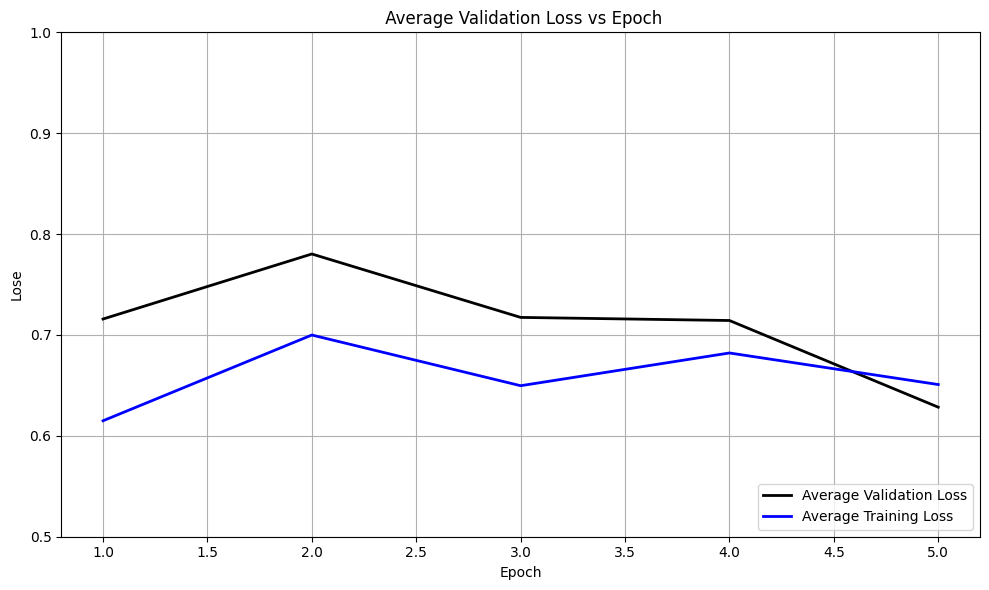
\includegraphics[width=0.8\textwidth]{figures/avg_loss.png}
	\caption{Average training and validation loss across folds.}
	\label{fig:atvlaf}
\end{figure}

\newpage
Figure~\ref{fig:cm_dl} shows the confusion matrix for the true class label and predicted class label after the training and validation. The matrix shows the correctly predicted male and female samples and their corresponding percentages. Females have slightly higher true positives compared to males in the number and percentages, which are 94 and 88, corresponding to 74\% and 69\%, respectively. Additionally, the falsely classified samples were 33 for females and 39 for males, respectively, accounting for 26\% and 31\%.

The results from the confusion matrix of the CNN model also matches what is observed in the descriptive statistics. Just like in the results from KNN, female samples again have slightly better correct classification rates. This can be explained by having lower variability in their morphometric attributes—particularly shell length, with females having a much smaller standard deviation (SD = 7.49) than males (SD = 31.75). This similarity probably makes the female class simpler to acquire and generalize for the model. Additionally, some shape-based ratios (for instance, UL ratio, UH ratio) that varied subtly but consistently by sex might provide sharper decision boundaries for females, particularly if the neural network is sensitive to subtle differences in spatial features. In contrast, the larger variation of male feature values may have caused intersections with female patterns and thus raised the rate of false negatives among males. This implies that although the deep learning model captures complex patterns, variability in features remains a source of error for reliable classification of the male class.

\begin{figure}[!htbp]
	\centering
	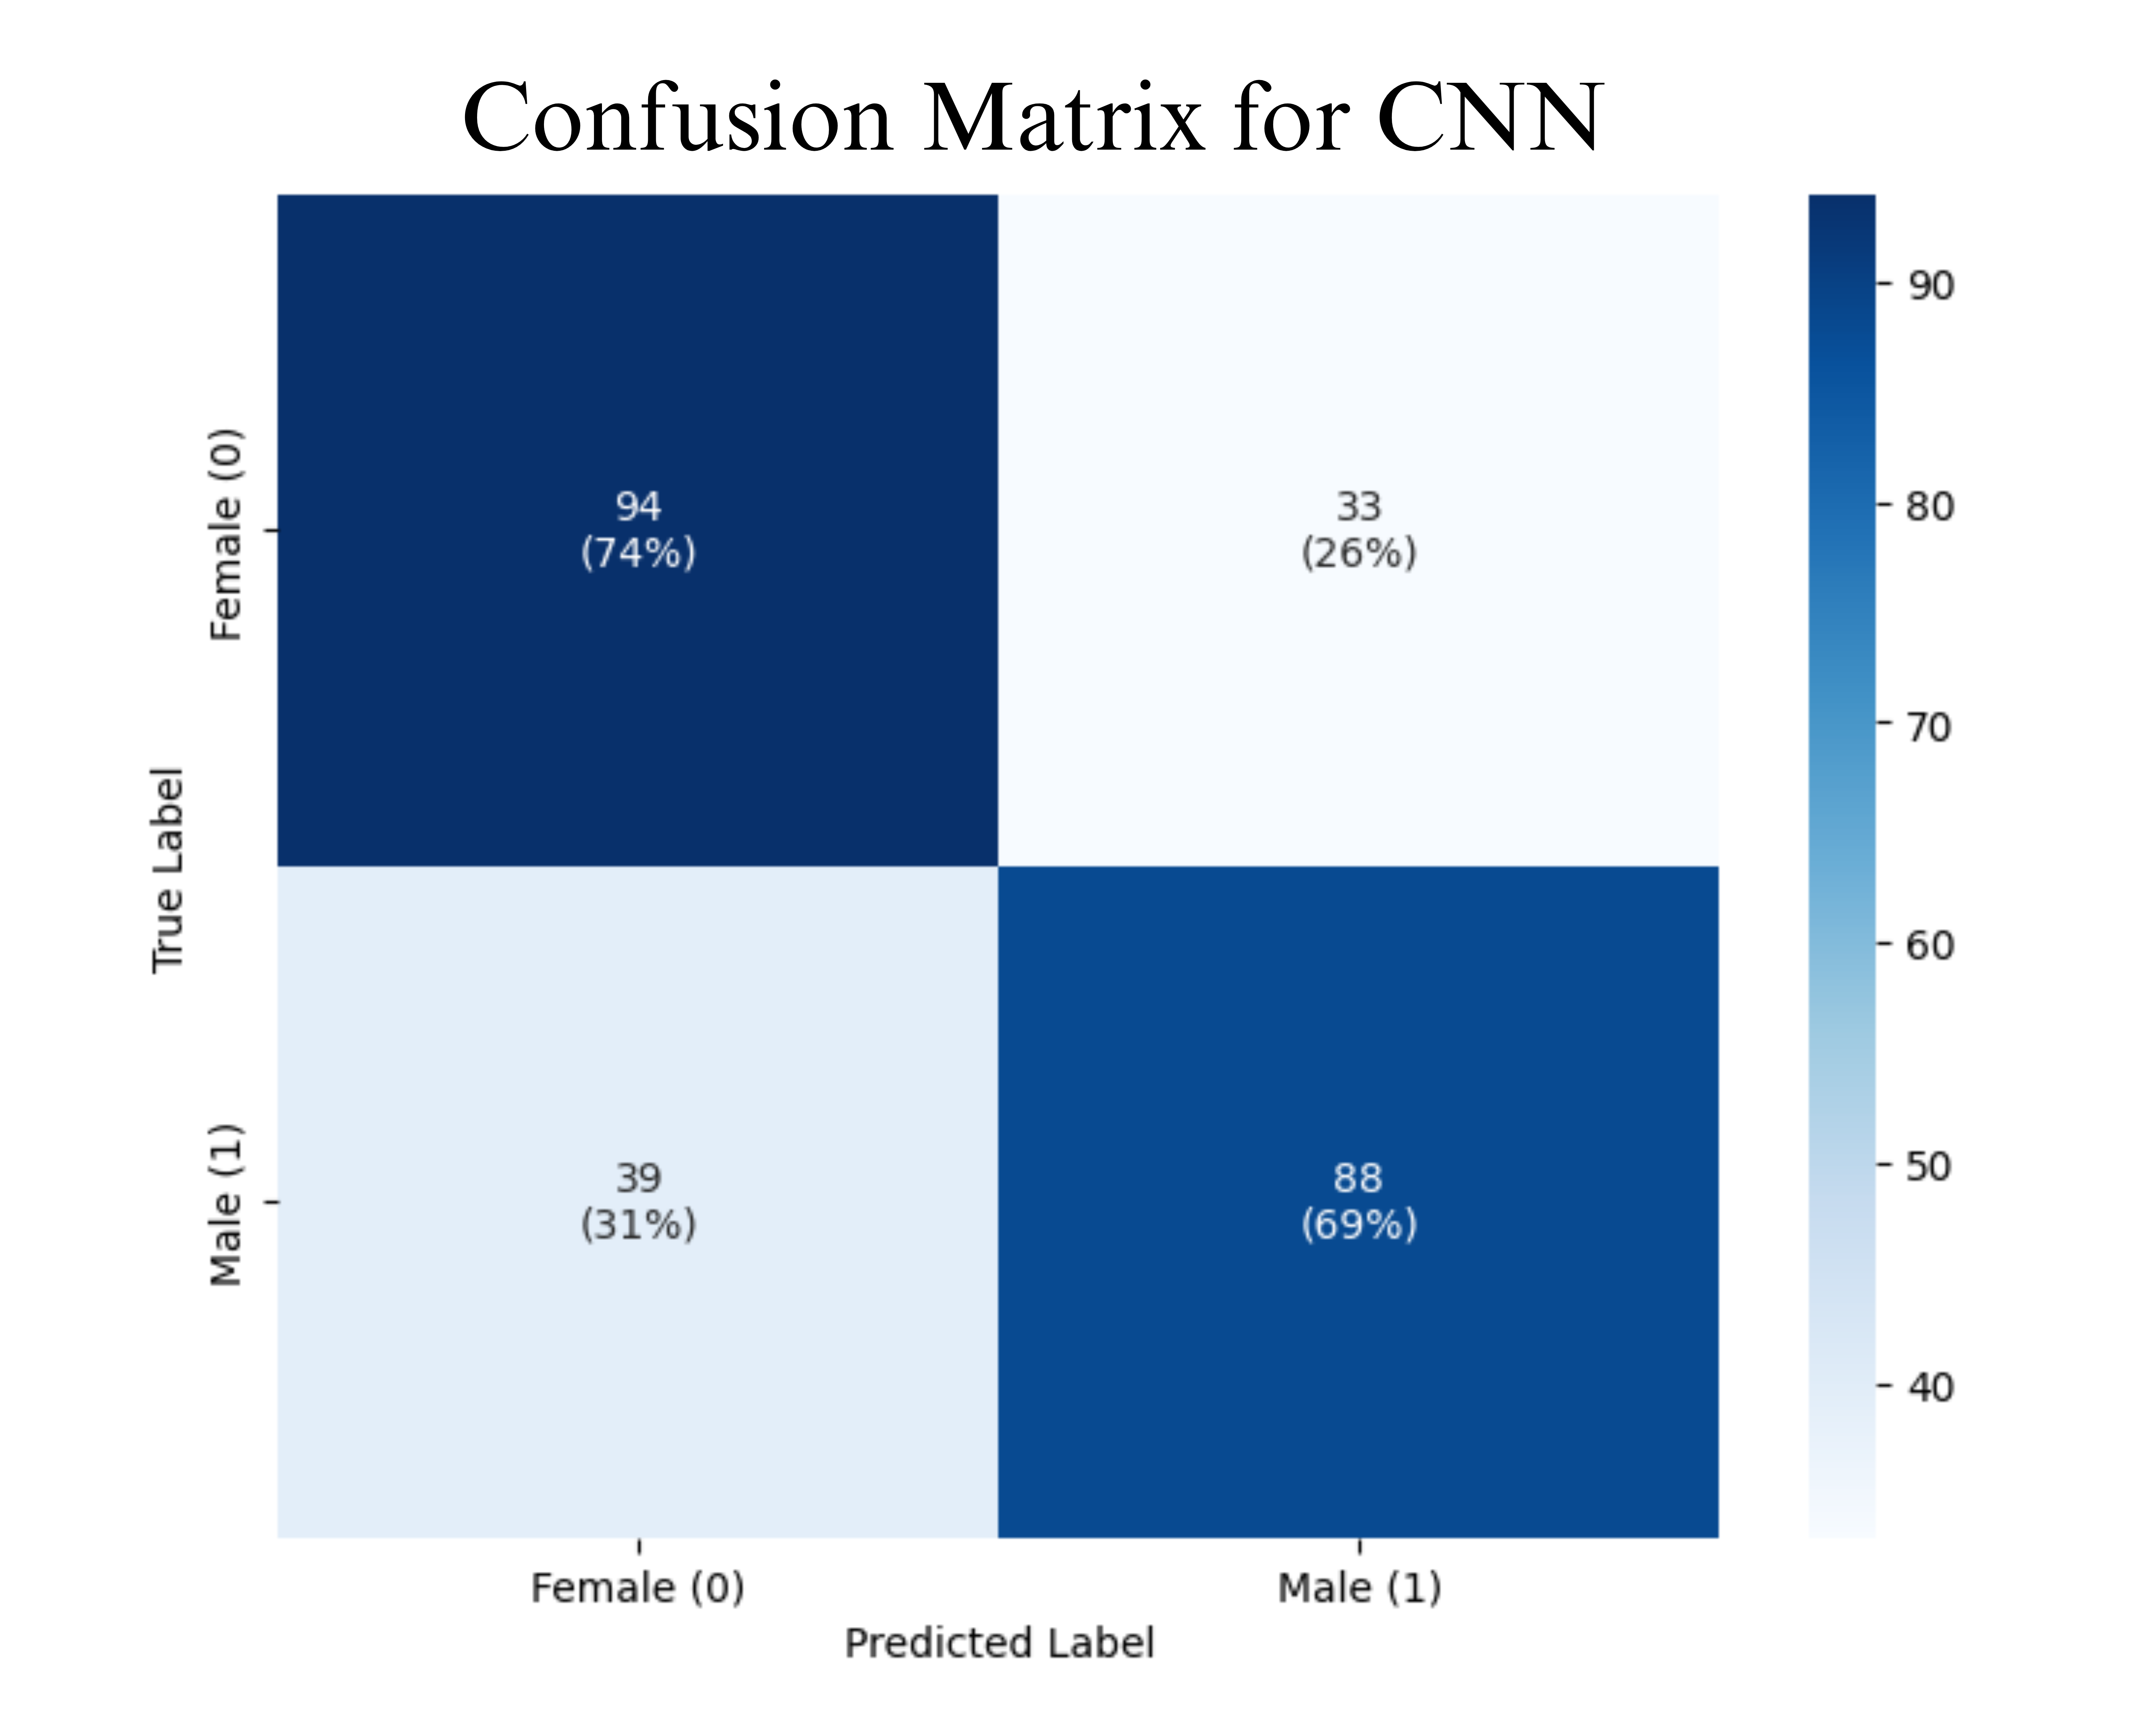
\includegraphics[width=0.8\textwidth]{figures/cm_dl.png}
	\caption{Confusion matrix for CNN model (Batch Size: 32, Epochs: 50, Activation Function: ReLU).}
	\label{fig:cm_dl}
\end{figure}

\newpage
Figure~\ref{fig:roc_auc} shows the average receiver operating characteristic (ROC) curve, showing the proposed model’s ability to correctly identify the true positives, which can help determine the trade-off between specificity and sensitivity. It will also determine the model's validity, supporting that it is not being predicted based only on random chance. The range of area under the receiver operating characteristic curve (AUC-ROC) is between 0.5 and 1. The model achieved an average score of 0.7734, which is better than random chance and a positive indication that the model is performing reasonably.

\begin{figure}[!htbp]
	\centering
	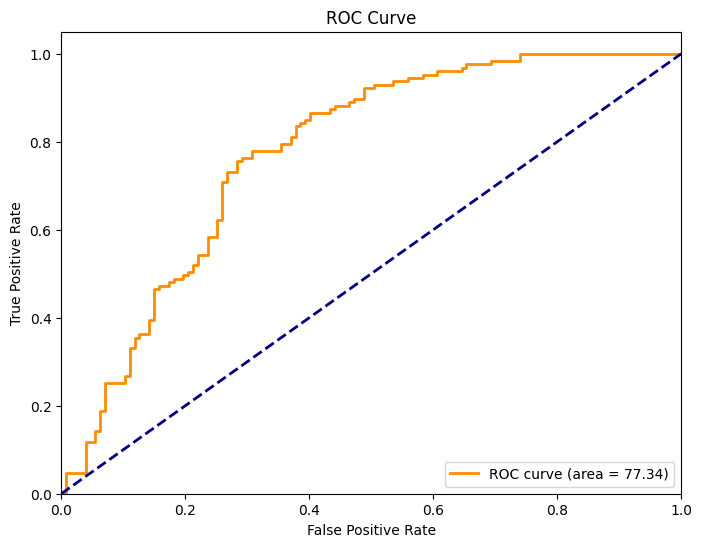
\includegraphics[width=0.6\textwidth]{figures/roc.png}
	\caption{ROC curve with area under the curve (AUC) score for the proposed model.}
	\label{fig:roc_auc}
\end{figure}

\newpage

\section{Discussions}

This study aimed to develop a noninvasive method for identifying the sex of \Tgranosa using machine learning and deep learning technologies. Specifically, it explored the relevance of linear shell measurements and image data in building accurate classification models that can support sustainable aquaculture practices.

In the machine learning experiments, feature selection played a key role in enhancing model performance. A reduced set of five statistically significant features, which were identified through Mann-Whitney U and Kruskal-Wallis tests, outperformed models using all available features. The k-nearest neighbors (KNN) classifier, trained on these five features, achieved an accuracy of 64.16\%, precision of 64.97\%, recall of 64.16\%, F1 score of 63.57\%, and an AUC-ROC score of 70.04\%. The width-height ratio observed from the left lateral view emerged as the most discriminative feature, with a correlation score of $p = 0.18$.

Deep learning experiments further revealed the impact of image angle and hyperparameter tuning on classification performance. The left lateral view consistently yielded the highest metrics, with the best model reaching 71.68\% accuracy, 72.52\% precision, 69.29\% recall, 69.12\% F1 score, and 77.34\% AUC using a batch size of 32 and 50 training epochs. Additionally, balanced dataset and activation function contributed to improved model performance.

The improved accuracy from models using fewer, more relevant features supports the idea that dimensionality reduction, when guided by statistical analysis, can enhance classification. The prominence of the left lateral view in both machine learning and deep learning results suggests that this angle reveals key morphological traits tied to sex differentiation. This aligns with the biological premise that some external characteristics may be more distinguishable when viewed from specific perspectives.

These findings demonstrates the feasibility of a noninvasive, accurate, and scalable approach to sex identification in \textit{T. granosa}. This is especially important in aquaculture, where traditional sex identification methods are often invasive or require specialized knowledge. By reducing the need for physical intervention, this approach promotes animal welfare and operational efficiency, potentially enabling real-time sex identification in aquaculture settings.

When compared to related work, such as the gender classification of Chinese mitten crabs using CNNs \cite{cui2020}, this study reflects both shared methodologies and important distinctions. While both utilized CNN architectures, differences in image resolution, dataset characteristics, and species-specific morphology may explain the performance gap which is 98.90\% in the crab study compared to 71.68\% in this study. The lower accuracy here likely reflects subtler morphological differences in \Tgranosa and limited dataset size.

Despite promising results, the study has several limitations. The dataset size (271 samples) was relatively small, which may have affected model generalizability. Additionally, image data was constrained to six fixed angles, potentially missing other informative views. These limitations may restrict the model’s effectiveness across diverse populations or environmental conditions.